\documentclass{sigchi}


\usepackage{graphicx}    % This package is used for Figures
\usepackage{balance} % to better equalize the last page
\usepackage{times}    % comment if you want LaTeX's default font
\usepackage{url}      % llt: nicely formatted URLs
\usepackage{rotating}

% llt: Define a global style for URLs, rather that the default one
\makeatletter
\def\url@leostyle{%
  \@ifundefined{selectfont}{\def\UrlFont{\sf}}{\def\UrlFont{\small\bf\ttfamily}}}
\makeatother
\urlstyle{leo}
% To make various LaTeX processors do the right thing with page size.
\def\pprw{8.5in}
\def\pprh{11in}
\special{papersize=\pprw,\pprh}
\setlength{\paperwidth}{\pprw}
\setlength{\paperheight}{\pprh}
\setlength{\pdfpagewidth}{\pprw}
\setlength{\pdfpageheight}{\pprh}

% Make sure hyperref comes last of your loaded packages, 
% to give it a fighting chance of not being over-written, 
% since its job is to redefine many LaTeX commands.
\usepackage[pdftex]{hyperref}
\hypersetup{
pdftitle={SIGCHI Conference Proceedings Format},
pdfauthor={LaTeX},
pdfkeywords={SIGCHI, proceedings, archival format},
bookmarksnumbered,
pdfstartview={FitH},
colorlinks,
citecolor=black,
filecolor=black,
linkcolor=black,
urlcolor=black,
breaklinks=true,
}

% create a shortcut to typeset table headings
\newcommand\tabhead[1]{\small\textbf{#1}}


\begin{document}

\title{Community Engagement and Community Response of First Time Code Contributors on GitHub}

\numberofauthors{2}
\author{
  \alignauthor 1st Author Name\\
    \affaddr{Affiliation}\\
    \affaddr{Address}\\
    \email{e-mail address}\\
    \affaddr{Optional phone number}
  \alignauthor 2nd Author Name\\
    \affaddr{Affiliation}\\
    \affaddr{Address}\\
    \email{e-mail address}\\
    \affaddr{Optional phone number}    
}

\maketitle                % create title and copyright pages

\keywords{
	open source; online communities; software development
}

\category{K.6.3.}{Management of Computing and Information Systems}{Software Management}

%%% Abstract %%%
\begin{abstract}           % abstract environment, this is optional
We collect data for 13,383 first time code contributions from 45 projects on the
website GitHub and analyze behavior of developers before submitting code as well
as community response to code contributions. We find that most developers do not
engage with the community on GitHub before attempting to submit code changes. We
also find that most code submissions do not elicit much community response, and
the metrics we use for community response can not predict whether or not a pull
request is accepted. Our findings differ from previous research on open source
software communities and social theories of learning in communities of practice.
\end{abstract}

\section{INTRODUCTION}

GitHub is a social website that open source software developers use to host
their software projects and to browse other developers' projects. It includes
many features that are present on social networking sites, such as the ability
to follow other users and leave comments on projects. GitHub provides a wealth
of data for studying computer supported cooperative work, as it is a
centralized location where many different tasks take place. For example, users
can create bug reports, submit fixes, and engage in discussions about new
features all on one website.

As open source software continues to grow and more users become reliant on open
source technologies, it is important to understand how this software is
developed. Research of open source software can also contribute to existing
research in a variety of other fields, including software engineering and computer
supported cooperative work. In this study, we examine the behavior of first time
code contributors and the community response to their code contributions. In
Section~\ref{sec:relatedwork}, we discuss how previous studies in open source
communities provide insight for existing literature on virtual teams and
distributed work. This study examines how new users join these types of
communities.

We are interested in how community engagement by a developer and community
response affects whether or not a first time code contribution is accepted or
not. We focus on code contributions as this shows the first time a user is
attempting to participate in a core act of development. Code contributions can
also be accepted or rejected, so our analysis allows us to see how these
social factors contribute to acceptance within the community.

The rest of this paper is organized as follows. The rest of this chapter
provides an overview of terminology specific to GitHub that will be used
throughout the paper, as well as  a literature review on research of communities
of practice and open source, establishing the importance of studying open source
software development, situating it within a context of virtual work and computer
mediated communication, and reviewing a theoretical basis we use to inform our
empirical methods. Chapter~\ref{chap:methods} describes our data collection and
data analysis methods. The results of our experiments are discussed in
Chapter~\ref{chap:results}. Our results differ from previous research in this
area. In Chapter \ref{chap:conclusion} we situate our findings in relation to
prior research and identify areas for future work.


\subsection{Terminology} \label{sec:terms}

A software project on the website is referred to as a \textit{repository}. Any
user on GitHub can \textit{star} a repository. Users star repositories to be
able to easily navigate to them and to receieve updates on activity from the
repositories. A repository can be private, meaning that it is only visible to
the owner and anyone the owner grants access to, or public, meaning that anyone
can view it. Our study focuses on public repositories. If a developer wants to
contribute to another one of developer's repositories, he can \textit{fork} the
repository, which creates a copy of the project for him to work on. As the
developer makes changes to this code, he \textit{commits} his changes. A
\textit{commit} is a snapshot of the code at a certain point in time. When the
developer is finished, he can submit a \textit{pull request} to the owner of the
project. All pull requests for a project are viewable on GitHub, and any user of
the site can comment on them. A pull request can have a status of open or
closed. A status of open indicates that that owner of the repository has not
made a decision about whether or not to include the changes. If the owner of a
repository wants to incorporate the changes the developer made, he can
\textit{merge} them into the repository. A pull request can be closed without
being merged, which means that the changes the developer made were not accepted.


\subsection{Related Work} \label{sec:relatedwork}

\subsubsection{FLOSS Research}
Research in the development of free/libre open source software (FLOSS) has grown
tremendously in the last several years.  Crowston et
al.~\cite{crowston_free/libre_2008} note the importance of understanding FLOSS
development as it becomes a major social movement with many volunteers
contributing to projects, and many FLOSS projects becoming integral parts of the
infrastructure of modern society. Other studies have emphasized the role that
FLOSS research can play in improving current existing research of software
engineering, particularly as the importance of understanding large scale
software systems in science and insustry increases
~\cite{scacchi_free/open_2007}.

Existing research approaches FLOSS from many different angles, including
motivation of open source
developers~\cite{fang_understanding_2009, lakhani_why_2003, shah_motivation_2006}; governance of open souce
projects~\cite{hippel_open_2003, omahony_guarding_2003, omahony_governance_2007};
and knowledge sharing within FLOSS
communities~\cite{endres_tacit_2007, hemetsberger_collective_2009, sowe_understanding_2008}.
Our study focuses on the behavior of first time contributors to FLOSS projects
and community response to their contributions. We build on previous studies that
describe the social processes of community
joining~\cite{ducheneaut_socialization_2005, huang_mining_2005, von_krogh_community_2003}. Given the
distributed nature of FLOSS development, our findings contribute to current
descriptions of virtual work and distributed teams.

Previous studies have used version control histories to verify learning
processes of new members in FLOSS projects~\cite{huang_mining_2005}. GitHub,
however, has not been extensively studied as it is a relatively new social
platform. Dabbish et al.~\cite{dabbish_social_2012} studied how GitHub as a
social application provides transparency and how that transparency affects
collaboration and learning. They found that this transparency leads to
inferences around commitment, work quality, community significance and personal
relevance, which supports collaboration and learning. McDonald and
Goggins~\cite{mcdonald_performance_2013} studed how different communities on
GitHub measure success, finding that most developers measure success in the
number of contributors and contributor growth. They also found that developers
believed the GitHub interface, in particular the use of pull requests, made
communities more democratic and transpartent. Choi et
al.~\cite{choi_herding_2013} studied a sample of GitHub based projects to
contribute to theories of developer coordination, finding that commits tend to
happen in clustered events over time. In all these cases, the social features of
GitHub, e.g. the ability to follow other users and view information about them,
provide new ways to study social behavior in FLOSS projects. Our study
investigates members' participation in group discussions on the site. While
previous studies have tried to combine data from mailing lists and version
control~\cite{ducheneaut_socialization_2005}, GitHub provides a centralized
location to study communities in which discussion and code contribution all
occur in one place. At least with regards to user support, recent research
suggests that developers may be moving away from mailing lists to social Q\&A
sites to respond to user requests for help~\cite{vasilescu_how_2014}. By
focusing on GitHub data, we contribute to understanding developer behavior on
this new social platform.


\subsubsection{Communities of Practice} \label{sec:communities}
Our study focuses on the behavior of new code contributors and community
response to their contributions. We use the theoretical framework of
\textit{legitimate peripheral participation} (LPP) ~\cite{lave_situated_1991} in
our exploration community joining. LPP describes a process of learning in
communities of practice in which newcomers join a community by participating in
peripheral tasks and forming relationships to move towards the center of the
community. Several studies of FLOSS development have used the LPP framework.
Huang and Liu~\cite{huang_mining_2005} mined version control history to
construct developer networks and identify core and peripheral community members.
Ducheneaut~\cite{ducheneaut_socialization_2005} found a pattern that resembles
LPP in his study of contributors to the Python project. Ye and
Kishida~\cite{ye_toward_2003} used LPP to ground their theory of motivation in
open source communities. This concept has been explored in other studies of
computer mediated communication.  In their study on members of Wikipedia, Bryant
et al. ~\cite{bryant_becoming_2005} note that members initially become involved
through peripheral activities. These are simple and low risk activities members
can take part in to learn more about the community before trying to become major
contributors. Similarly, von Krogh et. al ~\cite{von_krogh_community_2003} from
observing open source communities generated the construct of a \textit{joining
script}, where each project has a set of tasks for new developers to go through
before being accepted into the community.  The data we collect in
Section~\ref{sec:datacollection} is based on this theoretical framework. We
consider making code changes and submitting a pull request to be a core
activity, and commenting on other pull requests to be the primary peripheral
activity a user can participate in on GitHub. This follows previous studies that
find most users participate in community discussions prior to submitting
code~\cite{ducheneaut_socialization_2005, von_krogh_community_2003}.

\section{METHODS} \label{chap:methods}


\subsection{Data Collection} \label{sec:datacollection}

Data was collected using the GitHub API.\footnote{http://developer.github.com/}
We used a collection of node.js scripts to collect data from the API to store in
a MySQL database.\footnote{These scripts are available at
http://www.github.com/matthewheston/gh-collector.} In selecting which
repositories to use for our analysis, we started with the top 100 most starred
repositories on GitHub. We started with this list with the assumption that they
were popular repositories that would be maintained by an active community. From
these 100, we manually filtered out certain projects that we expected would
follow different development patterns than a typical programming project, for
example, collections of configuration files for text editors and shells,
collections of icons, etc. We also excluded repositories that were used
primarily for demonstration or documentation purposes, such as sample web
applications to demonstrate use of a certain web framework. After filtering our
intial list of 100, 45 repositories remained in our data set for analysis. We
consider only pull requests with a status of closed. This resulted in
approximately 44,400 pull requests. We further filtered this data by selecting
only the first pull request a user submitted to a repository, leaving 13,383
pull requests. The distribution of these pull requests across repositories
ranges from 10 to 1,489, with a median of 210. To find merged pull requests, we
first filter all pull requests that are marked as merged by the GitHub API,
meaning that the project maintainers used GitHub's merge feature to accept the
pull request. In some repositories, project maintainers use a different workflow
when accepting pull requests, wherein the code changes are accepted, but it is
not reflected as merged on GitHub. In most of these cases, there is a standard
way of reflecting this in the commit comments, so we use some naive heuristics
for identifying these requests by searching commit comments for certain text
patterns. For example, in many projects, the project maintainer will manually
add the commits from the pull request, and create a new commit with a commit
message that follows the pattern "Closes {number}" where {number} is the pull
request ID on GitHub. Finding merged pull requests using both the status from
the GitHub API as well as these text patterns results in finding 5,239, or
39.1\% of first pull requests being merged.

\subsection{Data Analysis} \label{sec:data_analysis}

We divide our analyis into two dimensions: community engagement of developer and
communtiy response. Our research questions our presented in
Table~\ref{tbl:research_questions}, along with a summary of the variables and
methods we used.

\begin{table*}[ht] \centering
\caption{Summary of research questions and methods.}
\label{tbl:research_questions}
\begin{tabular}{ p{2.1in} p{2.1in} p{2.3in} }
\hline\hline
Research Question
& Data                                  & Measure
\\
How does a user engage before submitting their first pull request?
& Comments on other pull requests.      & We plot the total number
of pull requests a user has commented in
Figure~\ref{fig:up_density}.
\\
Does community response affect whether or not a pull request is
merged? & Number of comments on pull request.   & We plot the
total number of comments for submitted pull requests in
Figure~\ref{fig:aprr_density}.
\\
~
& Language in comments on pull request. & We train both a
logistic regression and naive bayes classifier after
converting comments on submitted pull requests to feature
vectors. Results are shown in
Table~\ref{tbl:classifiers} \\
\hline
\end{tabular}
\end{table*}

\subsection{Community Engagement of Developer}
To explore the process of legitimate peripheral participation, we count the
total number of pull requests a developer commented on before submitting his own
pull request. As discussed in Section~\ref{sec:communities}, we consider
commenting on other pull requests the primary peripheral activity a user can
participate in. Previous studies indicate that users participate in technical
discussions before submitting code~\cite{von_krogh_community_2003}. Pull
requests allow users to comment on new features or other changes to the code
base. Although there are other peripheral activities a user may engage in on the
site, for example, making updates to a project wiki, not all projects use these
other features offered by GitHub. Pull requests are used by all the repositories
in our data set, so we examine only those comments to quantify participation by
a user. This variable is shown in Figure~\ref{fig:up}.

\begin{figure}[p] \centering
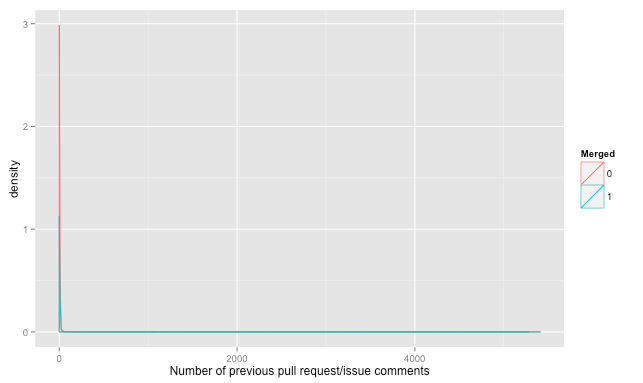
\includegraphics[scale=0.6]{figures/number_comments_density_ggplot.png}
\caption{User participation density plots.}  \label{fig:up}
\end{figure}

\begin{figure}[p] \centering
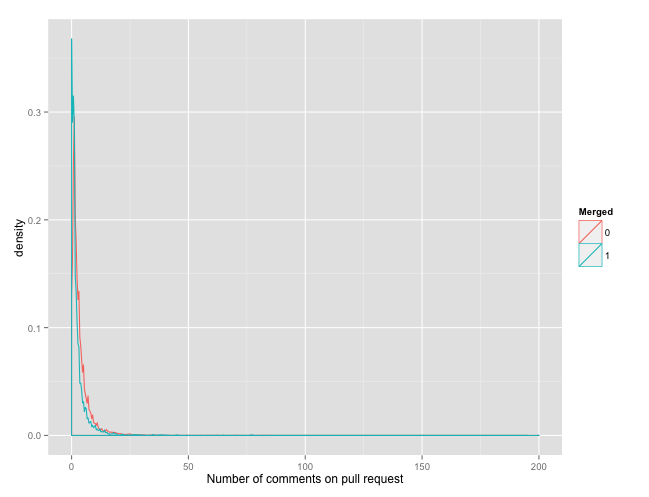
\includegraphics[scale=0.6]{figures/comments_on_pr_density_ggplot.png}
\caption{Attention pull request receives density plots.}  \label{fig:aprr}
\end{figure}

\subsection{Community Response}
In addition to measuring the activity of a developer in the community before
submitting a pull request, we are also interested in measuring the community
response to a given pull request and how that response relates to whether or not
a pull request is accepted. We measure this in two ways.

First, we simply count the number of comments on a given pull request. This is
used as a basic metric of how much attention a pull request receives. This
variable is shown in Figure~\ref{fig:aprr}.

Our next analysis of community response focuses on the language of the comments
on a pull request. To test whether or not the content of these comments is
predictive of whether or not a pull request is merged, we collect the comments
for each of our first pull requests. We ignore comments made by the user who
submitted the pull request, since we are interested in what other users had to
say about it. We also ignore the last comment associated with a pull request,
since these often will explicitly say whether or not the maintainer is merging
the pull request or not.  We are interested in whether the type of language used
in the discussion of a pull request is predictive of whether or not it is
accepted. We ignore pull requests that only have one comment associated with it.
This leaves 5,674 pull requests. Of these, 3,811, approximately 67\%, were not
accepted. We treat the remaining comments associated with the pull request as
one document, and convert them into feature vectors representing the count of
each unigram and bigram in the documents, and train both a logistic regression
and naive bayes classifier using this feature set. The results of testing these
classifiers is shown in Table~\ref{tbl:classifiers}. The results shown are the
result of running 10-fold cross validation.

\begin{table}[ht] \centering
  \caption{Classifier results}
  \label{tbl:classifiers}
  \begin{tabular}{lll}
  \hline\hline
  ~         & Logistic Regression & Naive Bayes \\
  Accuracy  & 69.6\%              & 70.6\%      \\
  Precision & 56.0\%              & 60.3\%      \\
  Recall    & 36.1\%              & 30.7\%      \\
  \hline
  \end{tabular}
\end{table}

\section{RESULTS} \label{chap:results}

\subsection{Community Engagement of Developer} \label{results_engagement}

We see that user participation for the majority of all first pull requests, both
merged and not merged, is 0. This indicates that in general, most users are not
attempting to engage in the peripheral activity of commenting on other pull
requests before submitting their own. The GitHub interface makes it relatively
easy for a user to fork a repository, make changes, and submit the changes for
consideration. Previous studies on GitHub have shown that the number of
contributions did increase for some projects that moved from other hosting
options to GitHub~\cite{mcdonald_performance_2013}. It is possible this
interface lowers the barrier of entry for a developer who wants to contribute to
a project, and allows them to bypass participating in the joining script
described by von Krogh et al. ~\cite{von_krogh_community_2003}.

We also examine these variables for first pull requests by users who later
submit another pull request. We want to see whether or not this ``no engagement"
pattern continues to hold for users who will become active contributors. Our
intuition here is that some users might encounter a bug they fix or desire a
feature that they implement, and then submit these changes back to repository.
They may not comment on other pull requests as they are not interested in
becoming long term members of the community, but rather are just interested in
submitting a one time patch. Users who do plan on becoming active members,
however, may participate in peripheral activities more.
Figure~\ref{fig:repeaters} shows a visualization of the same first pull
requests, but only for users who submit at least one other pull request at a
later point in our data set, and Figure~\ref{fig:repeaters_10} shows the data
for users who submit at least 5 more times. Looking at users who submit at least
one other time cuts our number of observations from 13,383 to 5,207, indicating
that approximately 61\% of these pull requests come from users who will not
contribute any others. Looking at users who will submit at least 10 more times
gives us a total of 1,155 observations.

It is clear that in all these cases, regardless of whether or not they will be
continuing to submit other pull requests later, at the time of submitting their
first pull request, users are generally not participating in the community. The
previous graphs only consider the number of pull requests a user commented on
before submitting their first pull request, so we do not capture how users who
submit multiple pull request over time comment on other pull requests over time.
In Figure~\ref{fig:commented_pullrequests_totals} we plot the total number of
others' pull requests that a user commented on by how many pull requests they
submitted themselves, considering only users who have submitted at least two
pull requests. There is not a strong correlation between these variables
(Spearman's $\rho$  = 0.44), indicating that users do not necessarily
participate in more commenting as they continue to submit more pull requests.

It's worth noting the one extreme outlier present in our data. One user
submitted pull request received 200 comments and was submitted by a user who had
commented on 900 previous pull requests. This is an interesting case of a
project maintainer, who has commit access and wouldn't typically need to submit
a pull request to submit changes, creating a pull request for commits related to
a major upgrade in the project. By creating a pull request, he was able to
document all the changes associated with this change and allow community members
to ask questions or comment on the changes. He has a high number of previous
comments since he is in charge of accepting pull requests. Due to the nature of
this pull request, there is a high number of comments on this pull requests on
it, since many other developers are asking questions or voicing their opinions.
This is a useful example that demonstrates the different ways pull requests may
be used in different projects, and how the way they are used may change
depending on the type of user submitting them.

\begin{figure}[p] \centering
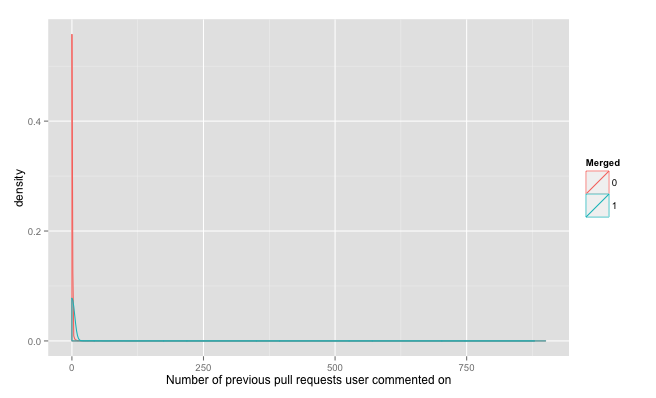
\includegraphics[scale=0.6]{figures/number_comments_density_repeaters_ggplot.png}
\caption{User participation density plots for users who submit at least one
other pull request in our data set.} \label{fig:repeaters} \end{figure}

\begin{figure}[p] \centering
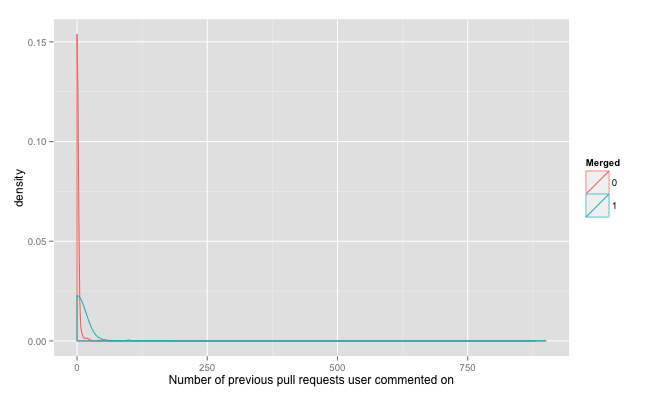
\includegraphics[scale=0.6]{figures/number_comments_density_repeaters_10_ggplot.png}
\caption{User participation density plots for users who submit at least ten
other pull requests in our data set.}
\label{fig:repeaters_10} \end{figure}

\begin{figure}[p] \centering
\includegraphics[scale=0.6]{figures/commented_pullrequests_totals_ggplot.png}
\caption{Total number of pull requests commented on and total number of pull
requests submitted for each user.} \label{fig:commented_pullrequests_totals}
\end{figure}

\subsection{Community Response}
In Figure~\ref{fig:up}, we see more variance in the number of comments on
first pull requests than we did with the number of pull requests users commented
on before submitting. However, this variable does not seem to be a good
predictor of whether or not a pull request is merged, since both the merged and
not merged distributions follow a similar pattern. It seems just viewing the
amount of activity a pull request receives is not enough to explain whether or
not it gets merged.

Training classifiers using the comment text may help address this problem, as
this can capture the valence of the comments, rather than just the raw number.
However, the low recall rates we see in Table~\ref{tbl:classifiers} indicate
that the text data is not sufficient to distinguish positive cases. We list the
top five features for each class in Table~\ref{tbl:features}. Despite leaving
out the last comment from each comment thread to avoid words that explicitly
describe the action being taken, we still see these in our top features. Both
"land" and "landed" are used in some repositories when a commit is merged, but
not through the GitHub interface to indicate the git commit hash where the pull
request commits were merged. We also see "closing" in the negative class, which
shows explicit action being taken. Some of our top features do seem fitting. The
phrase "lgtm" which stands for "looks good to me" seems indicative of positive
feedback from the community. Other examples, however, seem to indicate
overfitting, which we see in the top feature for the negative class, the word
"the."

Our sample size of 5,674 is relatively small, but it is interesting to note that
only 42\% of the first pull requests in our data set have more than 1 comment
associated with them. Our research question that drove these experiments was how
community response affects whether or not a pull request is accepted. However,
we see that the majority of pull requests don't attract any community attention.

\begin{table}[ht] \centering
\caption{Classifier top features}
\label{tbl:features}
\begin{tabular}{ll|ll}
\hline\hline
Merged  & ~     & Not merged  & ~      \\
land    & 0.817 & the         & -0.734 \\
landed  & 0.767 & bootstrap   & -0.711 \\
fine    & 0.717 & good thanks & -0.682 \\
lgtm    & 0.709 & in          & -0.682 \\
it will & 0.656 & closing     & -0.605 \\
\hline
\end{tabular}
\end{table}

\section{Conclusion} \label{chap:conclusion}

In this study, we analyzed community engagement and community response of first
time code contributors on GitHub. We found that most developers do not engage by
participating in discussions on GitHub before submitting code changes. We also
fou dthat most submitted pull requests do not attract much community response,
and our attempts at measuring community response did not provide good predictors
for whether or not a pull request is accepted. Our findings have implications
for researchers, open source contributors, and open source project maintainers.

We found that most users do not engage with the community in the way we expected
from previous FLOSS and LPP literature. Some reasons for this are discussed
below in Section~\ref{sec:future_work}. Since GitHub is a new platform that
encourages new types of social interactions, it can be used as a new source of
data to study open source communities. Our study focused on a relatively small
number of repositories pulled from the most starred repositories on GitHub.
Further work should be done on a larger sample of different types of
repositories. It's possible that new types of social websites like GitHub will
require new theoretical ways of thinking about distributed work and virtual
teams.

The majority of first pull requests in our data set were not accepted, but
community engagement is not a good predictor or whether or not they are
accepted, and most developers do not engage before submitting a pull request,
even if they end up becoming active code contributors. The implication for
developers who want to become involved in an open source project on GitHub is
that they do not necessarily need to participate in peripheral activities before
submitting pull requests. Although our study did not identify which factors do
contribute to acceptance of pull request, it's possible that developers should
focus more on things like finding relevant issues to fix or features to work on
rather than on social interactions.

Many open source projects fail due to insufficient volunteer
participation~\cite{crowston_defining_2003},~\cite{krishnamurthy_cave_2002}. It
is therefore important for project maintainers to continue to attract volunteer
developers to keep a project alive. We found that 61\% of first pull requests
in our data set come from users who will not submit any other pull requests.
Project owners should consider ways to convert these one time contributers to
regular active contributors.

Our major finding in this study is that, despite previous FLOSS research which
did indicate social patterns that follow legitimate peripheral participation
framework~\cite{ducheneaut_socialization_2005, huang_mining_2005, ye_toward_2003},
we generally do not see this pattern in our GitHub data set. Although some
developers do leave comments on other pull requests before submitting their own,
the majority of developers do not, including those that will continue to submit
code changes. There are many reasons this might be the case.

As mentioned in Section~\ref{results_engagement}, GitHub's interface makes it
fairly easy to submit changes. Users only need to click a button to create a
copy of the repository that they can make commits on, and then click another
button to submit those commits as a pull request when they are finished. This
process may lower barriers to entry for new developers. While previous studies
of FLOSS communities have focused on mailing lists and centralized version
control repositories, the distributed nature of git may be altering the social
patterns that take place in developer networks. This study may suggest we need
to alter existing social theory as new interfaces change social interactions.

\subsection{Limitations of the Study} \label{sec:limitations}

This study only focused on data from GitHub, and our notion of community
engagement by developers was limited to activity by developers on GitHub. While
we have shown that this data is not sufficient to predict whether or not a pull
request is merged, further studies should create joint data sets merging GitHub
data with data from other sources, such as mailing lists, forums, or chat rooms
to test whether or not developers engage with the community using these other
platforms, and how those social interactions affect their acceptance in the
community. One difficulty in creating these types of data sets is identify
merging, the process of matching different logins from different services to the
same physical person, but a number of techniques have been proposed to assist in
this process~\cite{bird_open_2007, goeminne_comparison_2013, kouters_whos_2012}.
We also focused only used pull request comments to measure community engagement
by a developer. Other GitHub features, such as issues and wikis, provide other
ways to participate in a repository that we did not cover.

It is also important to note that the GitHub platform is used in different ways
across projects. As described in Section~\ref{sec:datacollection}, there was
some work required to identify merged pull requests due to the different ways a
project maintainer accepts the pull request, e.g. through the GitHub interface
or not. In Section~\ref{results_engagement}, we discuss an outlier in our data
where a user who did not typically contribute code through the pull request
mechanism did use this feature in order to allow community feedback and
questions. There are many other examples in differences in use of the GitHub
platform. Some projects, for example, may require all developers to submit pull
requests for the purposes of code review, while others may grant commit access
to certain developers that allows them to bypass the pull request mechanism.
Although we did account for differences in accepting pull requests, there may be
other nuances across projects that affect the data we collected that are harder
to detect when working with data at scale.

\subsection{Future Work} \label{sec:future_work}

In examining community engagement and community response, our study was
primarily concerned with social factors within open source software development
communities. It's possible that looking at only social factors is not enough to
understand what contributes to acceptance on GitHub. Static analysis tools may
be used in addition to the metrics we used in this study to further explore how
the code itself affects whether or not a pull request is accepted.

In studying how communities respond to pull requests, we found in most cases, there was little
community response. As mentioned above, attraction of new developers and
retention of developers is important to project success. Future work should how
community response can affect developer retention in GitHub projects.

In examining the top features for the classifiers we trained in studying
community response, we found some issues. Our goal in filtering the text
collected was to avoid words that explicitly described action being taken. We
still found examples of these types of words in both our positive and negative
classes. In the case of the positive (merged) class, the top feature was
"land." This feature affects classifier performance since this word is used
often in positive cases, but only in a few repositories. Future work studying
linguistic features in this way should account for these types of project
specific vocabularies.

Finally, to better understand the way that the GitHub interface affects
developer behavior will require further qualitative study. While there have been
surveys of GitHub developers previously~\cite{mcdonald_performance_2013}, there
remains a lot of work left to do in this area. Future quantitative studies
should collect larger samples of data and explore new ways of measuring these
types of social variables.

\subsection{Conclusion}

In this study, we measured community engagement and community response of first
time code contributors to GitHub. Using data from the pull request feature of
GitHub, we studied how developers engage open source communities before
contributing code, as well as how community response to these code contributions
predicts whether or not they are accepted. We found that most users do not
participate in other social GitHub features before submitting code.  In
attempting to measure community response, we found that most code contributions
do not receive much communtiy response, and that both the raw amount of comments
on a GitHub pull request as well as the language in those comments were not good
predictors of whether or not the pull request is accepted.

%
% BIBLIOGRAPHY
%
\bibliographystyle{acm-sigchi}
\bibliography{Master}
\end{document}
